\documentclass[11pt]{report}
\usepackage{dina4}
\usepackage{eurosym}
\usepackage{fontspec}
\usepackage[sc]{mathpazo}
\setmainfont[Ligatures=TeX]{Palatino Linotype}
\usepackage{fancyvrb}
\usepackage[table]{xcolor}
\usepackage{floatpag}
\floatpagestyle{empty}
\definecolor{linkcolor}{rgb}{0,0,0.5}
\usepackage[colorlinks=true,linkcolor=linkcolor,citecolor=linkcolor,filecolor=linkcolor,pagecolor=linkcolor,urlcolor=linkcolor]{hyperref}
\usepackage{tikz}

\usepackage{xeCJK}
%\setCJKmainfont[BoldFont=STZhongsong, ItalicFont=STKaiti]{STSong}
%\setCJKsansfont[BoldFont=STHeiti]{STXihei}
%\setCJKmonofont{STFangsong}


\def\xyzemail{xingyuanzhang at 126 dot com}
\def\cwemail{chunhanwu at 126 dot com} 
 
   
\begin{document}
\title{\LARGE\bf ITP 2015 Conference Booklet}
\author{Xingyuan Zhang, Chunhan Wu  and Christian Urban}
\date{\today}
%%\tableofcontents 
\maketitle

\chapter{Pre-Arrival}

\section{Registration and Conference Fee}

In short

\begin{itemize}
\item[(1)] you need to make a bank transfer for the conference 
fee in your local currency, and  
\item[(2)] you need to email Xingyuan with your details 
  (\xyzemail)
\end{itemize}

\noindent Xingyuan will then confirm that the payment has been
received. Note that if you are Chinese and need a \emph{fa
piao} to reclaim the conference fee, you need to contact 
Xingyuan directly before making any money transfer. 
\medskip
 
\noindent The early conference fee is RMB 3300, which is
approximately \pounds{}350, \$533, or \euro{}488. It must be
transferred via bank transfer and must be made in your local 
currency; we cannot accept any other form of payment. The 
tutorials can be registered independently from the conference. 

The conference fee includes lunches during the conference. It
also covers the excursion, the conference banquet and a
welcome reception. 

\begin{center}
\begin{tabular}{l@{\hspace{4mm}}l}
Early conference fee until 31.~July: & RMB 3300\\
Late conference fee from 1.~August:  & RMB 3800\bigskip\\

Additional banquet dinner and excursion: & RMB 530\\
(one is included in the conference fee)\bigskip\\

Isabelle tutorial (21 -- 23 August): & RMB 250\\
Coq tutorial (27 -- 29 August):       & RMB 200\\
\end{tabular}
\end{center}

\noindent The amount payable needs to be
transferred to the account:

\begin{center}
\begin{tabular}{ll}
Account holder's name:&  Zhang Xingyuan\medskip\\

Beneficiary bank:& BANK OF CHINA\medskip\\

Swift Code:& BKCHCNBJ940\medskip\\

Account number:& 504066588897\medskip\\

Beneficiary bank address:&   Nanjing Mei Hua Shan Zhuang\\ 
                         &    Sub-branch, Nanjing, China\medskip\\

Account holder's address:& \\
  & Suite 2106, Building 20,\\
  & 20 Biao Ying,\\ 
  & Qinhuai District,\\ 
  & Nanjing, Jiangsu Province,\\
  & People's Republic of China.\\
\end{tabular}
\end{center}

\noindent {\bf Please make doubly-sure that your bank
transferral contains your full name as reference (additional
information field), and is in your local currency 
(e.g.~\euro, \$, \pounds)!} Otherwise we will have no idea 
where the money came from, and will not be able to receive
the money on our end. Please also make sure that your transferral
covers all bank fees.\bigskip


\section{Hotel Booking}


In short, you need to send your arrival and departure 
details to Chunhan 
(\cwemail).\bigskip

\noindent While it is possible to book the hotel via official
online travel web-pages, the price there is higher. The
easiest is to send Chunhan your name, arrival and departure
dates and he will send you back a booking ticket from Hanyuan
hotel, which you might need for your visa application. 
You can pay the hotel when you arrive using Visa or
MasterCard.

\section{Visa}

Please be aware that for travelling to China you will need a
visa, for which you have to apply {\bf beforehand}. It often takes
one or two weeks before a visa is granted. Though if you 
are prepared to pay a higher application fee, then you can 
shorten the delay to a few days. For the visa you
will need an invitation letter, which Chunhan will send you
(\cwemail). You need to provide him with your name, title, 
DOB, work address, e-mail and paper title (if you present a paper). 
He will e-mail you the invitation letter. You might also need
your hotel booking (see above) and flight details for the visa
application.



\chapter{Arrival}

Welcome in China. You made it to the destination airport.
Unless your are one of the very few foreigners who can speak
and read Chinese, potentially the most challenging part of
your journey is about to begin. Below we explain how to get to
Hanyuan Hotel in Nanjing from Nanjing Lukou Airport and from
Shanghai Pudong Airport. If you arrive from somewhere else and
need help, please let us know. If you need help while 
travelling, the local organisers can be reached on their 
mobile:

\begin{center}
\begin{tabular}{ll}
Xingyuan: & (+86)\hspace{2mm}13814081536\\
Chunhan:  & (+86)\hspace{2mm}15312993807\\
\end{tabular}
\end{center}

China is generally a safe country for travelling, if the usual
precautions are taken. We assume you have never been in China 
before, therefore let us still start with some general points.

\begin{itemize}
\item \textbf{Weather}\hspace{3mm} 
Unfortunately end of August is the time when it will be especially
hot in Nanjing (usually above 30$^{\circ}$C). Be prepared with lots of
light clothes, but do not forget a jumper, or sweater, since many
places are air-conditioned. It can also rain.


\item \textbf{Bottled Water}\hspace{3mm}
Whereas in many places it is safe to drink water from taps,
do not take chances and drink only bottled water! During the
conference we will provide bottled water. In other places you
have to buy bottles yourself. Remember, Chinese are famous for
nibbling on a bottle of hot tea the whole day, even in sweltering 
temperatures. There is a reason for this. 

\item \textbf{Traffic}\hspace{3mm} 
Do not even think of renting a car in China. Hence, while in
China, you probably will be mostly going around on foot. Be
careful though: You might come from a region where traffic
rules are organised so that pedestrians are mostly treated
with respect by all other road users, or even have an
``elevated status'' because they are considered the
``weakest''. Traffic in China is, in contrast, organised more,
shall we say, according to a Darwinian model: Under no
circumstance assume a car (or even a bicycle or one of the
many noiseless electric motor bikes) will stop for you. As
pedestrian, you have to take care of everybody else.
Therefore, whenever possible cross roads at traffic lights and
even if the light shows green for you, look out for cars that
pay no attention to this fact. Also, zebra crossings do
\emph{not}, I repeat, \emph{do not} have any special meaning
in China for the road users higher up the traffic ladder
(i.e.~bicycles and above). Even if it sounds too funny, take
our word and heed this advice\ldots{}it might increase your
life-expectancy. 

\item \textbf{Free Public Wifi / Mobile Phones}\hspace{3mm}
While free public wifi is nowadays pretty ubiquitous in big
cities in China (Starbucks, Costas, McDonalds are obvious
places where to find wifi), you need nearly always a working mobile phone in
order to use it. You will have to register your number when
you log in, and the wifi operator will then send you a
password token via SMS. The problem is that chances are great
your mobile phone will \emph{not} work in China. Therefore do
not assume you can check information on the Internet while
travelling. 

At the hotel there will be wifi (named HanYuan-\_\_\_\_ with the super-secure
password: 123456789). But again, do not assume you can
download that last episode of the Daily Show: while bandwidth
will generally be enough for reading email, be prepared for an
uninterrupted stay in China, free from any disturbance coming
from online demands.
   
\item \textbf{Google etc}\hspace{3mm}There are two Great Walls in
China: one prevents you from accessing Google, for example. Use
\url{www.aol.com} or \url{www.bing.com} instead as your preferred
search engine. Also, if you care about such things, set your 
status on Facebook to ``unavailable'' for the period of time
you will be in China. Ditto Twitter. Skype and Facetime, in 
contrast, work fine. Dropbox, no.

\item \textbf{Map of Hotel / Taxis}\hspace{3mm} 
While more and more young Chinese are exposed to English, you
cannot rely on anyone of the general public speaking more than
a few words. Rather, you have to always calculate with the
very, very likely scenario that nobody speaks any English at
all and all signs around you are written in characters that do
not give you the slightest idea what they are about. This
means you always have to prepare your travelling beforehand
and ask us for help if you are unsure! 

One part of \emph{every} trip preparation, including your
arrival, should be to carry with you a printed copy of the map
where the Hanyuan Hotel is located (see Fig.~\ref{hanyuan}).
When you want to go to the hotel by taxi, you need to show the map to
the driver, since telling Hanyuan Hotel will most probably not
be understood and also the driver most likely does not know
where it is located. Showing the map will also guard against
the possible situation where a taxi driver cannot actually
read the address.\footnote{You might sneer at this. But
remember: the prime age of Chinese taxi drivers appears to be
50 plus. If you can also remember, between 1966 and 1976
somebody had the ``great'' idea to be nasty to teachers
(amongst others). So the education these people were able to
receive when they were in their teens was rather rudimentary.
Given that the ability of reading Chinese characters takes
years of arduous studying, it is glaringly obvious that it is
not their fault.} Take the map always with you: it might be
your life-line for avoiding unpleasant situations. For 
travelling inside Nanjing, taxis can be hailed at the
street curb. You need to pay them in cash. They are always
metered.

%There is a slight chance you will come across one of the all 
%electric taxi, which are slightly more expensive, than ``normal''
%taxis. You can recognise them as they are the only taxis built
%by the maker BYD and look more like a compact SUV, rather than
%the ``normal'' sedan-style taxi. I have not driven yet in one,
%but have seen them in the Xinjiekou shopping area. If you do not
%want to pay the additional price tag, you are assumed to just
%wave them away and wait for the next taxi.

\item \textbf{Tips in Restaurants, Taxi}\hspace{3mm}One easy
aspect of travelling in China are matters to do with tipping:
no tips are expected when paying at a restaurant, for a taxi 
journey etc. The good thing about this is you are treated as a 
nice customer, if you are a nice customer (meaning you treat 
staff with respect).

\item \textbf{Cash / Credit Cards}\hspace{3mm}While foreign
credit cards are accepted in a number of places, including
the hotel,\footnote{Visa and Mastercard} these places are 
considered ``upmarked'' in China. So if you insist on being able
to use your credit card, you will often be paying some form of 
premium. Cash still rules many aspects of Chinese life
(metro ticket, taxi journey,\ldots{}) where foreign credit cards 
are of no use (China has its own credit card system which is
accepted more widely, but also not everywhere). Pretty much the 
only places where cash can be obtained with a foreign credit 
card are ATMs in Chinese banks. There are several not far
from the hotel.
\end{itemize}

\begin{figure}[p]
\begin{tabular}{l}
For the driver:\medskip\\

司机师傅,请将我送到``{\bf 童卫路20号翰苑宾馆}'',其位置如地图中红色A点所示。\\
酒店电话:02584393962。谢谢!
\end{tabular}

\begin{center}
\makebox[0mm]{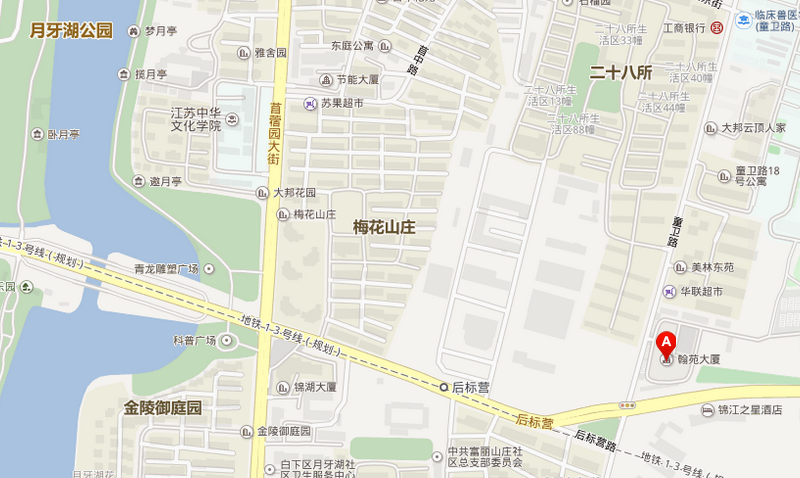
\includegraphics[scale=0.5]{travel_guide/badu.png}}
\end{center}
\caption{The location of the Hanyuan Hotel. Please print out!
\label{hanyuan}} 
\end{figure}
 


\section{Travel from Nanjing Lukou Airport to the Hanyuan Hotel}

There are essentially three options to travel from the Nanjing
Airport to the hotel depending on how frugal or adventurous
you want to be:

\begin{itemize}
\item The first option is to take a taxi for the whole journey
      from the airport to the hotel. Follow the taxi signs at
      the airport and take a yellow taxi. The journey will
      cost you around 130 RMB (\euro{}19, \$21) and takes
      about 45 minutes. Show the driver the map in
      Fig.~\ref{hanyuan}. The taxi needs to be paid in cash.
      Make sure the taxi driver switches on the meter once 
      you left the airport! 

\item A bit less expensive is going first by Metro Line S1
      from the airport to Nanjing Nan Railway Station (Nanjing
      South Railway Station). The metro will operate between
      6:40 and 22:00. As you can see in the map shown in
      Fig.~\ref{metronanjing}, Nanjing Nan will be the last
      stop on Line~S1. At Nanjing Nan Railway Station you need to go
      to the taxi stand, which means leaving the metro via exit 
      2B and follow the signs for ``Taxi (Underground)''.
      The way is marked yellow in the map below. 
      This option takes approximately
      55 minutes and costs 7 RMB for the metro ticket and
      around 36 RMB for the taxi.\\[-10mm]\mbox{}

      \begin{center}
      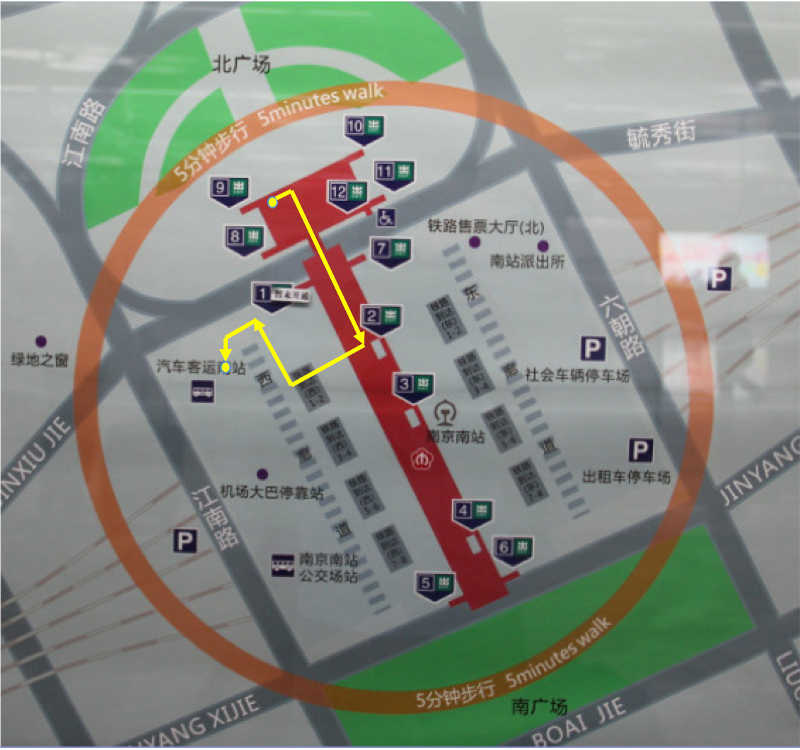
\includegraphics[scale=0.19]{travel_guide/ggg.jpg}
      \end{center}

\item If you already prepared to pay 7 RMBs for the metro, why
      not adding 2 more and going the whole way by metro? 
      This is the third
      option. The disadvantage is that you need to change
      at Nanjing Nan Railway Station to Line 3 and at 
      Daxinggong to Line 2 for Xiamafang or Muxuyuan, which
      are the closest stations to the Hanyuan Hotel 
      (see Fig.~\ref{metronanjing}). Both
      stations then need a 15 minutes walk to the hotel.
      This is another disadvantage of this option if you have 
      a heavy suitcase. See the map shown in Fig.~\ref{hotelmap}
      for directions between the metro stations and the
      hotel.
 \end{itemize}

\begin{figure}[p]
\begin{center}
\makebox[0mm]{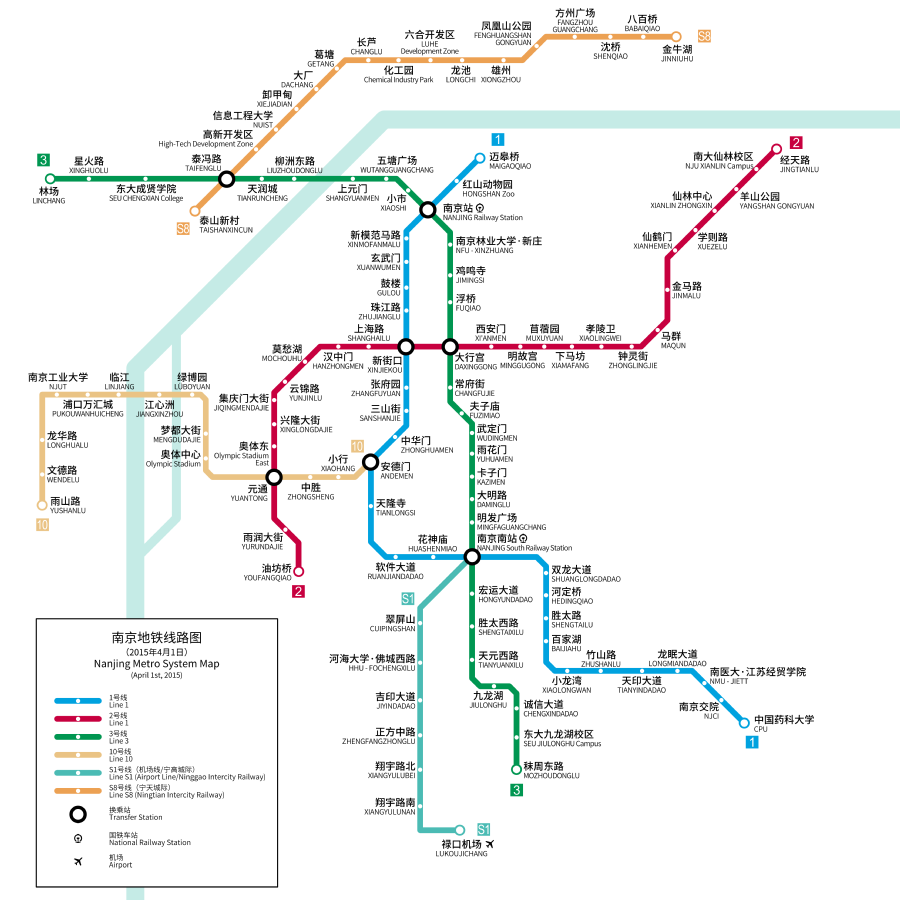
\includegraphics[scale=1.1]{travel_guide/metromapnanjing.png}}
\end{center}
\caption{Metro map of Nanjing. Stations
Xiamafang and Muxuyuan on Line 2 (red line) are 
closest to the hotel.\label{metronanjing}} 
\end{figure}

\subsubsection*{Getting a Ticket for the Metro in Nanjing}

Like most Chinese metro stations, entering the metro station
at the airport means you have to go through a brief security
check where your luggage will be X-rayed. After the check you
will see ticket machines

\begin{center}
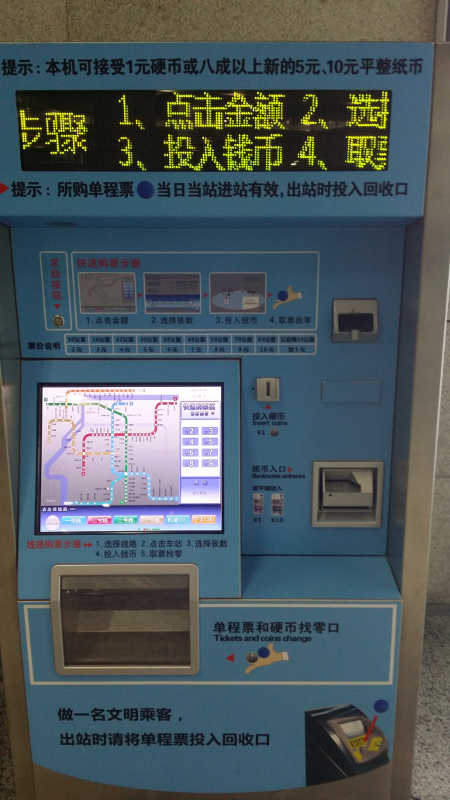
\includegraphics[scale=0.27]{travel_guide/20150331_110412.jpg}
\hspace{4mm}
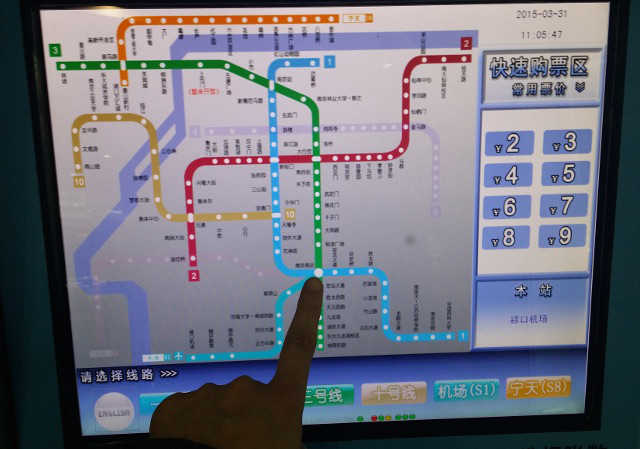
\includegraphics[scale=0.27]{travel_guide/20150331_110548.jpg}
\end{center}

\noindent which can change the language to English (in this
way you can avoid having to talk to a sales person in the ticket 
counter, who might not speak any English). You need to select 
the destination station on the touch screen (shown on
the right). Next you need to pay for the ticket with 10 RMB or 5
RMB bank notes, or 1 RMB coins. If you do not have them yet,
you will need to get your ticket from the counter.
After paying, the machine will issue a blue plastic chip which
is your ticket. This chip needs to be swiped when going
through the gates of the metro (shown on the right below). 
At the end of your journey you will have to return the blue 
chip at the exit gate.

\begin{center}
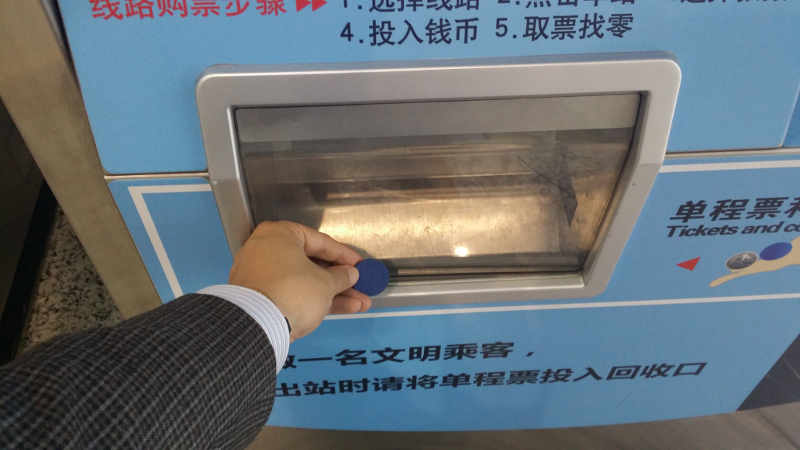
\includegraphics[scale=0.27]{travel_guide/20150331_110738.jpg}
\hspace{4mm}
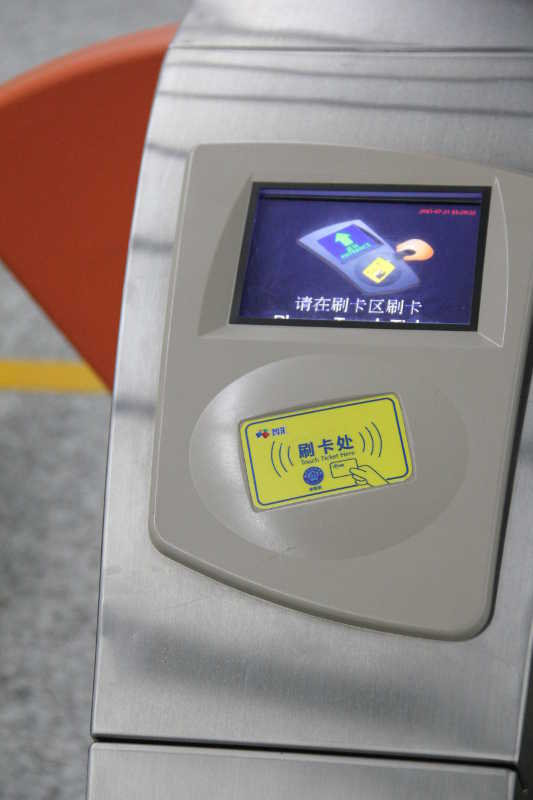
\includegraphics[scale=0.27]{travel_guide/IMG_7177.jpg}
\end{center}


\section{Travel from Shanghai Pudong Airport}

Many of the participants will arrive at Shanghai Pudong
Airport. From there, in short, you have to get to (1) the Hong
Qiao railway station and then from there to (2) Nanjing Nan
railway station. From Nanjing Nan it is best to take a taxi,
but you can also take the metro as explained in the previous
section. Overall this will take approximately 4h of travelling
to the hotel. 

\subsection*{From Shanghai Pudong Airport to Hong Qiao Railway Station}

For the first leg to Hong Qiao train station there are
essentially two travel options: one recommended by locals
and being the more sensible option is to take the airport bus;
the other is by the World's only commercial Maglev train 
including a change to the metro. 

\begin{itemize}
\item \textbf{Option 1 by Airport bus}: 
At the Pudong Airport follow the signs for Airport Bus, or
Airport Ring Bus. You have to take Line 1, which operates
between 7:00 and 23:00. The bus stop where you have to wait is 

\begin{center}
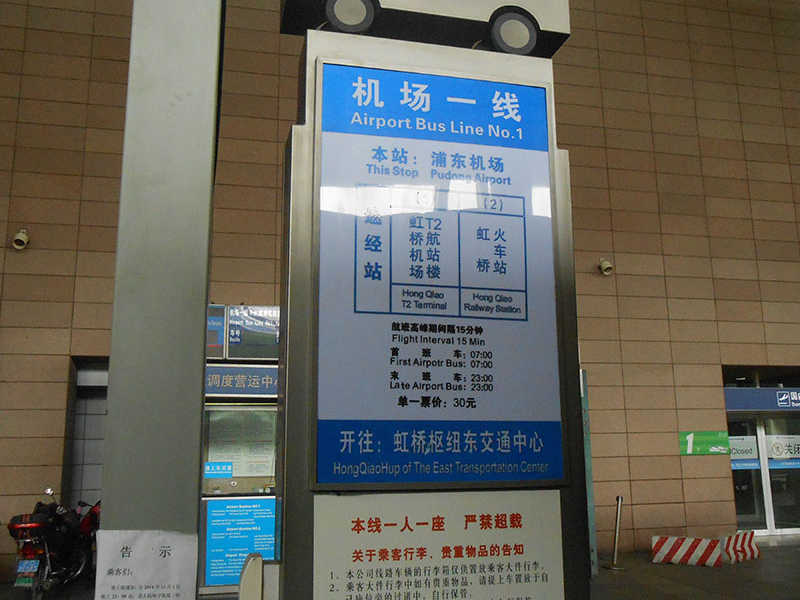
\includegraphics[scale=0.9]{travel_guide/image005.jpg}
\end{center}

The waiting time is around 15 minutes during peak hours, or 30
minutes at other times. The ticket costs 30 RMB (\euro{}4.25,
\$5) and can be bought on the bus. This however requires cash.
While you wait, be prepared to be harassed by taxi drivers,
who insist on driving you to Hong Qiao train station. You can
ignore them: it will cost you more, around 100 RMB; the bus is
comfortable and air-conditioned, unlike the taxi; and, like
the taxi driver, the bus driver appears to aim for maximum
possible speed given good road conditions. 


The airport bus takes around 1h and makes only two stops at
the very end of the journey. Both stops are in near
proximity. You have to take the \emph{second} stop at Hong Qiao
Railway Station. You will be able to see the big signs of
Hong Qiao Railway Station when you approach the station. Do 
not take the exit for Hong Qiao International Airport.

\item \textbf{Option 2 Maglev train / Metro}: 
Of course travelling on the Maglev is pretty cool\ldots{}
reaching speeds of 415 km/h at certain(!) times of the day,
namely 9:02--10:47 and 15:02--16:47. At other times it will
travel at mere speeds of 300 km/h, which you get in China also
with conventional high-speed trains. Anyway, a ticket for the
Maglev will set you back around 50 RMB (\euro{}7, \$8). The
ticket can be paid in cash or by credit card. The service of
the Maglev starts at 7:02 and finishes the day at 21:42. To
take this option at the airport, you will need to follow the
Maglev signs. The main problem with this option, however, is
that you can only travel until Longyang Road Station and then
have to change into the overcrowded and much, much slower
metro Line 2. The change to the metro is a short walk from the
Maglev. You have to first buy a ticket inside the metro
station. The good thing about this option is that metro
travelling in Shanghai is pretty easy for foreigners as all
stations are sign-posted in letters. For buying a ticket for
the metro, check the section about buying a metro ticket in
Nanjing (the procedure is pretty universal in China; the only
exception is that in Shanghai the metro ticket is a paper
ticket, while in Nanjing it is a blue plastic chip).

Overall the journey time of this option is around 2h. So
unless you really want to sample the feeling of travelling for
7 minutes at 415 km/h, we recommend Option 1 by bus.
\end{itemize}

\subsection*{From Hong Qiao Train Station to Nanjing Nan via
High-Speed Train}

The airport bus will stop directly in front of the southern
part of the Hong Qiao Railway Station. As background, train
stations above the village level in China are organised more
like an airport, than the more sleepy train station you might be
familiar with. Therefore, you first have to go through a
security gate where luggage is checked and you padded by a
security guard. The security guard might be of either sex and
this is seen as normal by Chinese. 

Next you need to buy a train ticket. There are ticket
counters, see left below, sign-posted in the main hall. (Unlike
the metro, ticket machines for trains are of no use for you,
because you would need a Chinese ID-card in order to buy
anything with them.)

\begin{center}
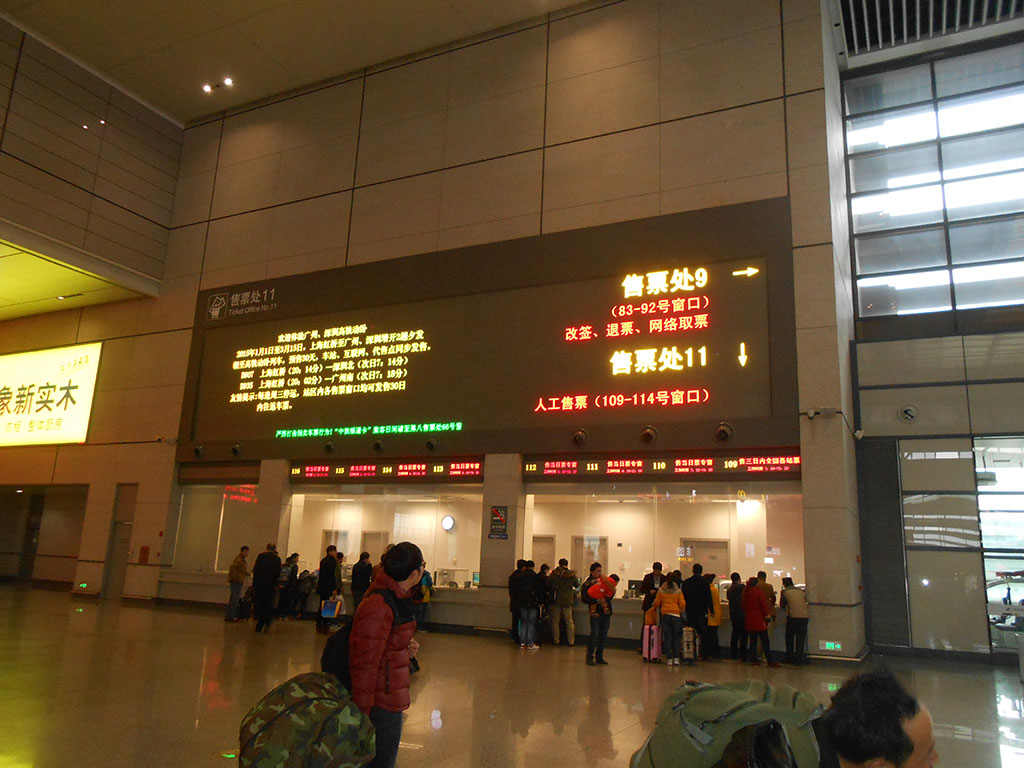
\includegraphics[scale=0.8]{travel_guide/image038.jpg}
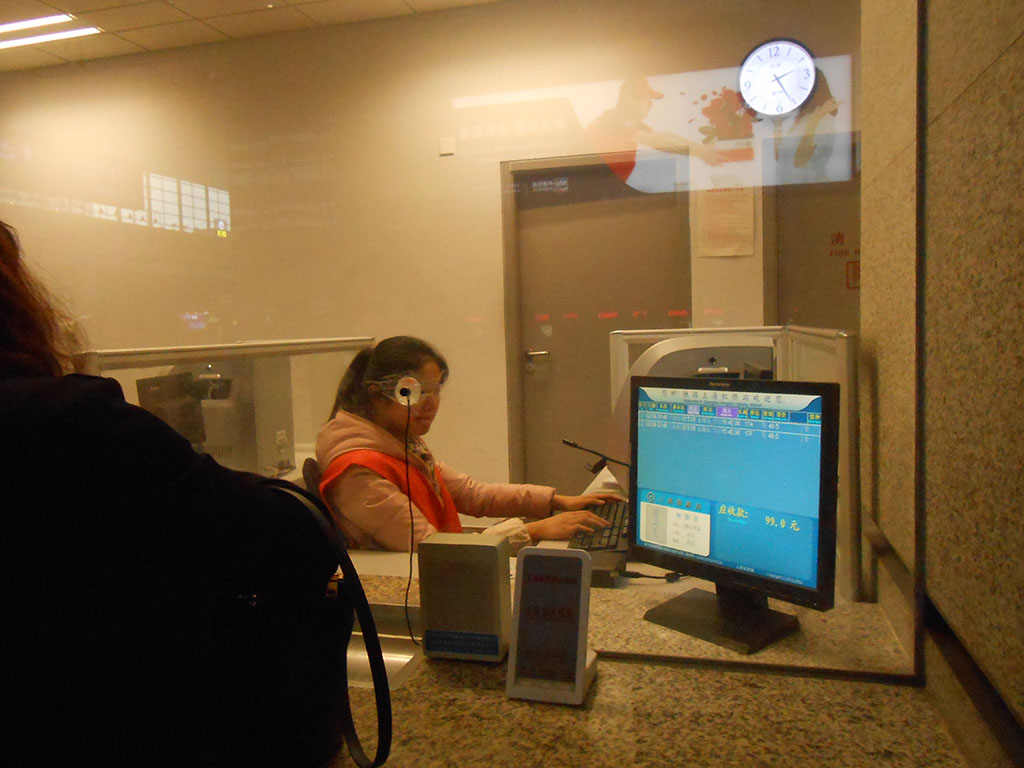
\includegraphics[scale=0.8]{travel_guide/image040.jpg} 
\end{center}

\noindent You have to queue on the usually longer queue and
buy a ticket for Nanjing Nan (Nan stands for South station).
You will need to show your passport in order to buy a ticket.
The ticket will cost around 135 RMB and looks like this:

\begin{center}
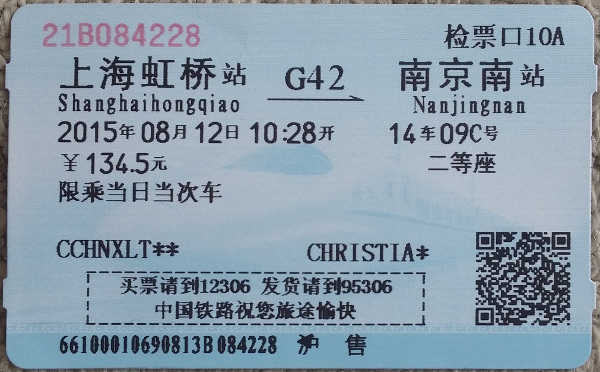
\includegraphics[scale=0.3]{travel_guide/ticket.jpg}
\end{center}

\noindent The G-Number (G42 above) stands for the train
number, which identifies the train also on the large displays
at the hall. Below that number is the date and departure time,
in this case 2015-08-12 and departure time 10:28. To the right
is the coach number (14) and seat number (09C). Just below
from that is the sign that the ticket is for second class (二). 
For the short duration of the trip there is no real need
to buy a ticket for first class. On the top right-hand corner
is the platform written (10A). If not, you have to look
at the large display in the hall to get this information.

Next you have to wait for your train on the main concourse of
the station. Assuming you have some time, rest for a moment
and take in the atmosphere of a typical Chinese train
station\ldots{} definitely busy. Once you know the
platform, go to the gate. Be careful, the gates are nestled
between shops and can be easily overlooked. For each platform
there are two gates labelled `A' and `B', respectively. They
are on opposite sides of the main hall. `A' stands for the
front of the train and `B' for the rear -- you know which one
to go to from the coach number on your ticket. When the gates
are opened for your train, you need to show again your passport
verifying that it is you who is travelling on the ticket. The
journey to Nanjing Nan takes around 1h.

\subsection*{Nanjing Nan Railway Station to the Hanyuan Hotel}

Like in the section for travelling from Nanjing Lukou Airport,
there are two options you can take from Nanjing Nan. The only
difference is that the train station has a different taxi
stand, which is sign-posted at the station. At the taxi stand
you need to take a yellow taxi that goes to ``Nanjing
Downtown''. The taxi will cost around 36 RMB and needs to be
paid in cash. Show the driver the map in Fig~\ref{hanyuan}.

%weather, electrical connectors
%% when does the welcome reception start?
%% breakfast needs more coffee

\chapter{Conference}

\section*{Overview}

\begin{center}
  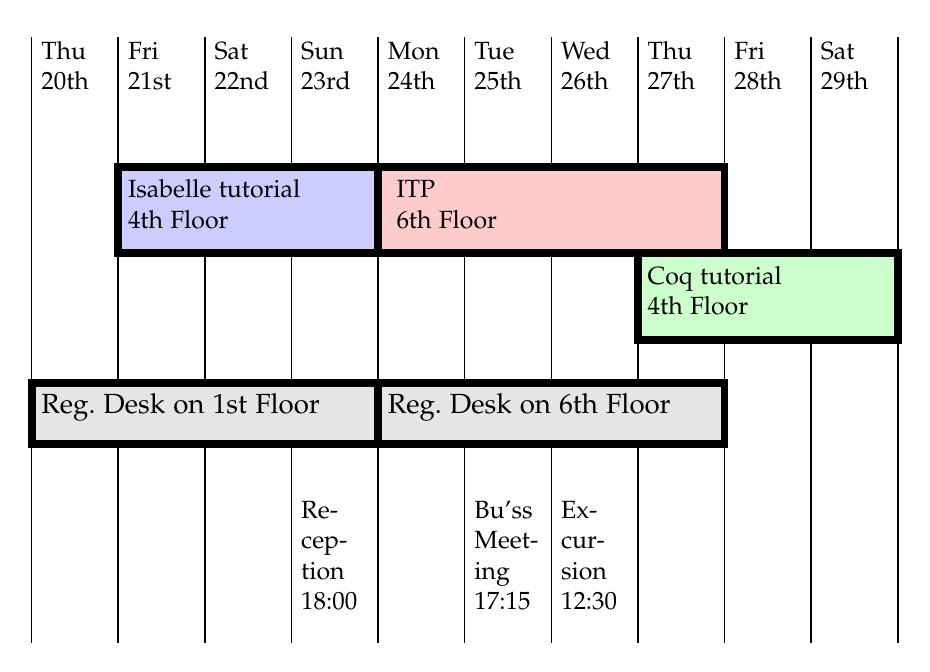
\begin{tikzpicture}[scale=1.1]
  %\draw[step=1cm] (0,-0) grid (10,6);
  
  \draw[line width=0.2mm] ( 0,-1.0) -- ( 0,6);
  \draw[line width=0.2mm] ( 1,-1.0) -- ( 1,6);
  \draw[line width=0.2mm] ( 2,-1.0) -- ( 2,6);
  \draw[line width=0.2mm] ( 3,-1.0) -- ( 3,6);
  \draw[line width=0.2mm] ( 4,-1.0) -- ( 4,6);
  \draw[line width=0.2mm] ( 5,-1.0) -- ( 5,6);
  \draw[line width=0.2mm] ( 6,-1.0) -- ( 6,6);
  \draw[line width=0.2mm] ( 7,-1.0) -- ( 7,6);
  \draw[line width=0.2mm] ( 8,-1.0) -- ( 8,6);
  \draw[line width=0.2mm] ( 9,-1.0) -- ( 9,6);
  \draw[line width=0.2mm] (10,-1.0) -- (10,6);
  
  \draw ( 0,6.1) node[anchor=north west] 
  {\small\begin{tabular}{@{}l}Thu\\ 20th\end{tabular}};
  \draw ( 1,6.1) node[anchor=north west] 
  {\small\begin{tabular}{@{}l}Fri\\ 21st\end{tabular}};
  \draw ( 2,6.1) node[anchor=north west] 
  {\small\begin{tabular}{@{}l}Sat\\ 22nd\end{tabular}};
  \draw ( 3,6.1) node[anchor=north west] 
  {\small\begin{tabular}{@{}l}Sun\\ 23rd\end{tabular}};
  \draw ( 4,6.1) node[anchor=north west] 
  {\small\begin{tabular}{@{}l}Mon\\ 24th\end{tabular}};
  \draw ( 5,6.1) node[anchor=north west] 
  {\small\begin{tabular}{@{}l}Tue\\ 25th\end{tabular}};
  \draw ( 6,6.1) node[anchor=north west] 
  {\small\begin{tabular}{@{}l}Wed\\ 26th\end{tabular}};
  \draw ( 7,6.1) node[anchor=north west] 
  {\small\begin{tabular}{@{}l}Thu\\ 27th\end{tabular}};
  \draw ( 8,6.1) node[anchor=north west] 
  {\small\begin{tabular}{@{}l}Fri\\ 28th\end{tabular}};
  \draw ( 9,6.1) node[anchor=north west] 
  {\small\begin{tabular}{@{}l}Sat\\ 29th\end{tabular}};

  \draw[line width=1mm,fill=blue!20] (1,4.5) rectangle (4,3.5);
  \draw[line width=1mm,fill=red!20] (4,4.5) rectangle (8,3.5);
  \draw[line width=1mm,fill=green!20] (7,3.5) rectangle (10,2.5);
  \draw (1,4.5) node[anchor=north west] 
  {\small\begin{tabular}{@{}l}Isabelle tutorial\\4th Floor\end{tabular}};
  \draw (4.1,4.5) node[anchor=north west] 
  {\small\begin{tabular}{@{}l}ITP\\6th Floor\end{tabular}};
  \draw (7,3.5) node[anchor=north west] 
  {\small\begin{tabular}{@{}l}Coq tutorial\\4th Floor\end{tabular}};

  \draw[line width=1mm,fill=gray!20] (0,2.0) rectangle (4,1.3);
  \draw[line width=1mm,fill=gray!20] (4,2.0) rectangle (8,1.3);
  \draw (0,2.0) node[anchor=north west] {Reg.~Desk on 1st Floor};
  \draw (4,2.0) node[anchor=north west] {Reg.~Desk on 6th Floor};
  
  \draw ( 3,0.8) node[anchor=north west] 
  {\small\begin{tabular}{@{}l}Re-\\cep-\\tion\\18:00\end{tabular}};
  \draw ( 5,0.8) node[anchor=north west] 
  {\small\begin{tabular}{@{}l}Bu'ss\\Meet-\\ing\\17:15\end{tabular}};
  \draw ( 6,0.8) node[anchor=north west] 
  {\small\begin{tabular}{@{}l}Ex-\\cur-\\sion\\12:30\end{tabular}};
  \end{tikzpicture}
\end{center}

\noindent Our registration desk will be on the 1st Floor next
to the hotel's registration desk from Thursday to Sunday. From
Monday, we will move the desk to the 6th floor where the
conference hall is. The registration desk is open from 9:00
until 17:00, except on Thursday 20th when it will open from
14:00 and on Monday 24th when it will be open from 8:15. In
case you arrive when our registration desk is closed, you can
still check into the hotel simply by showing your passport and
refer to ITP 2015. The hotel has a list of everyone who made a
booking. When you check into the hotel, they will ask for a
deposit to be reserved on your credit card. You will get back 
this deposit at the end of your stay (assuming you do not
trash your room in the meanwhile). \bigskip

\noindent The Welcome Reception on Sunday 18:00 will be on the
1st Floor. Breakfast and lunches are served on the 1st Floor
next to the hotel registration desk. The breakfast buffet is
open from 7:00 until 9:00. When you check into the hotel, you
will receive a green paper ticket for each day, which you have
to show before going to breakfast. For lunches you have to show
your ITP badge. Hanyuan Hotel also includes a quite good
restaurant on the 2nd floor, where you can have dinner and lunch.

\begin{itemize}
\item\textbf{Near the Hotel}\hspace{3mm}
The Hanyuan hotel is located at the intersection of a big 
road
(Houbiaoying Road 后标营路) and a smaller road (TongWei Road 童卫路).
If you need a taxi to go to Downtown Nanjing, for example, it
is probably the easiest to hail down a taxi at the big road.
An ATM machine is situated a few minutes walk down the smaller
TongWei Road. If you want to take a walk in the evening,
Xingyuan suggests a stroll through the Purple Mountain Area 
indicated on
the top-right in the map in Fig.~\ref{hotelmap}. This area is
approximately a 15 minutes walk away from the hotel and
contains for example the Sun Yat Sen memorial and the Linggu
pagoda (below right).

\begin{center}
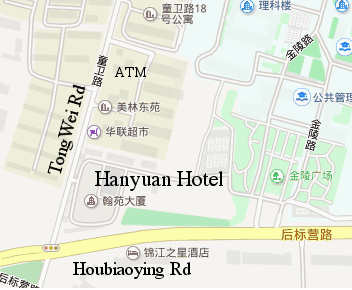
\includegraphics[scale=0.40]{travel_guide/map1a.jpg}
\hspace{5mm}
\includegraphics[scale=0.38]{travel_guide/linggusu.jpg}
\end{center}

\item\textbf{Metro Stations Near the Hotel}\hspace{3mm}
There are two metro stations near the hotel (Mu\-xuyuan and
Xiamafang stations), which are pretty much the same distance
from the hotel (see map in Fig~\ref{hotelmap}). Muxuyuan is
easier to reach: just down TongWei Road and then turn left
down the hill of NingHang Road (宁杭公路). The entrance of the
metro is on the left-hand side. However it is not the most
scenic route. More scenic is the walk to Xiamafang Metro
Station through the campus of the Nanjing Agriculture
University. Unfortunately the way is not so straightforward.
If you are unfamiliar with the way, we suggest you walk to
Muxuyuan station; once you followed a local and know the
way, go to Xiamafang Station.

\begin{figure}[p]
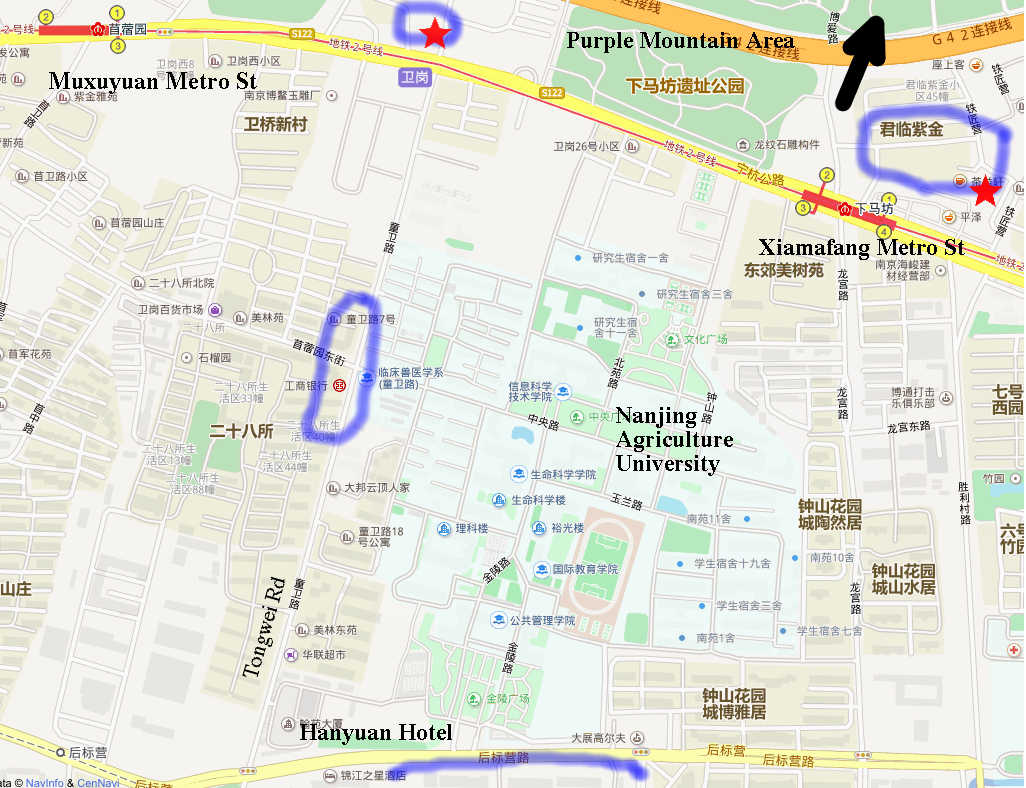
\includegraphics[scale=0.45]{travel_guide/map2.jpg}
\caption{Shops and restaurants in the vicinity of the hotel.
A relatively large shopping area including a large supermarket
(indicated with a red star)
is near the Xiamafang metro station. A smaller
supermarket is at the end of Tongwei Road. Another
shopping area including restaurants are in the middle of 
Tongwei Road. There are also restaurants on the big
Houbiaoying Road.
\label{hotelmap}}
\end{figure}

\item\textbf{Shops and Restaurants Near the Hotel}\hspace{3mm}
There is a relatively large shopping area close to Xiamafang
Metro Station. There is also a wide selection of restaurants
in this area including Xingyuan's favourite restaurant for
having lunch on workdays. It is called Changjinglu 
(meaning giraffe) and situated behind the KFC.

\begin{center}
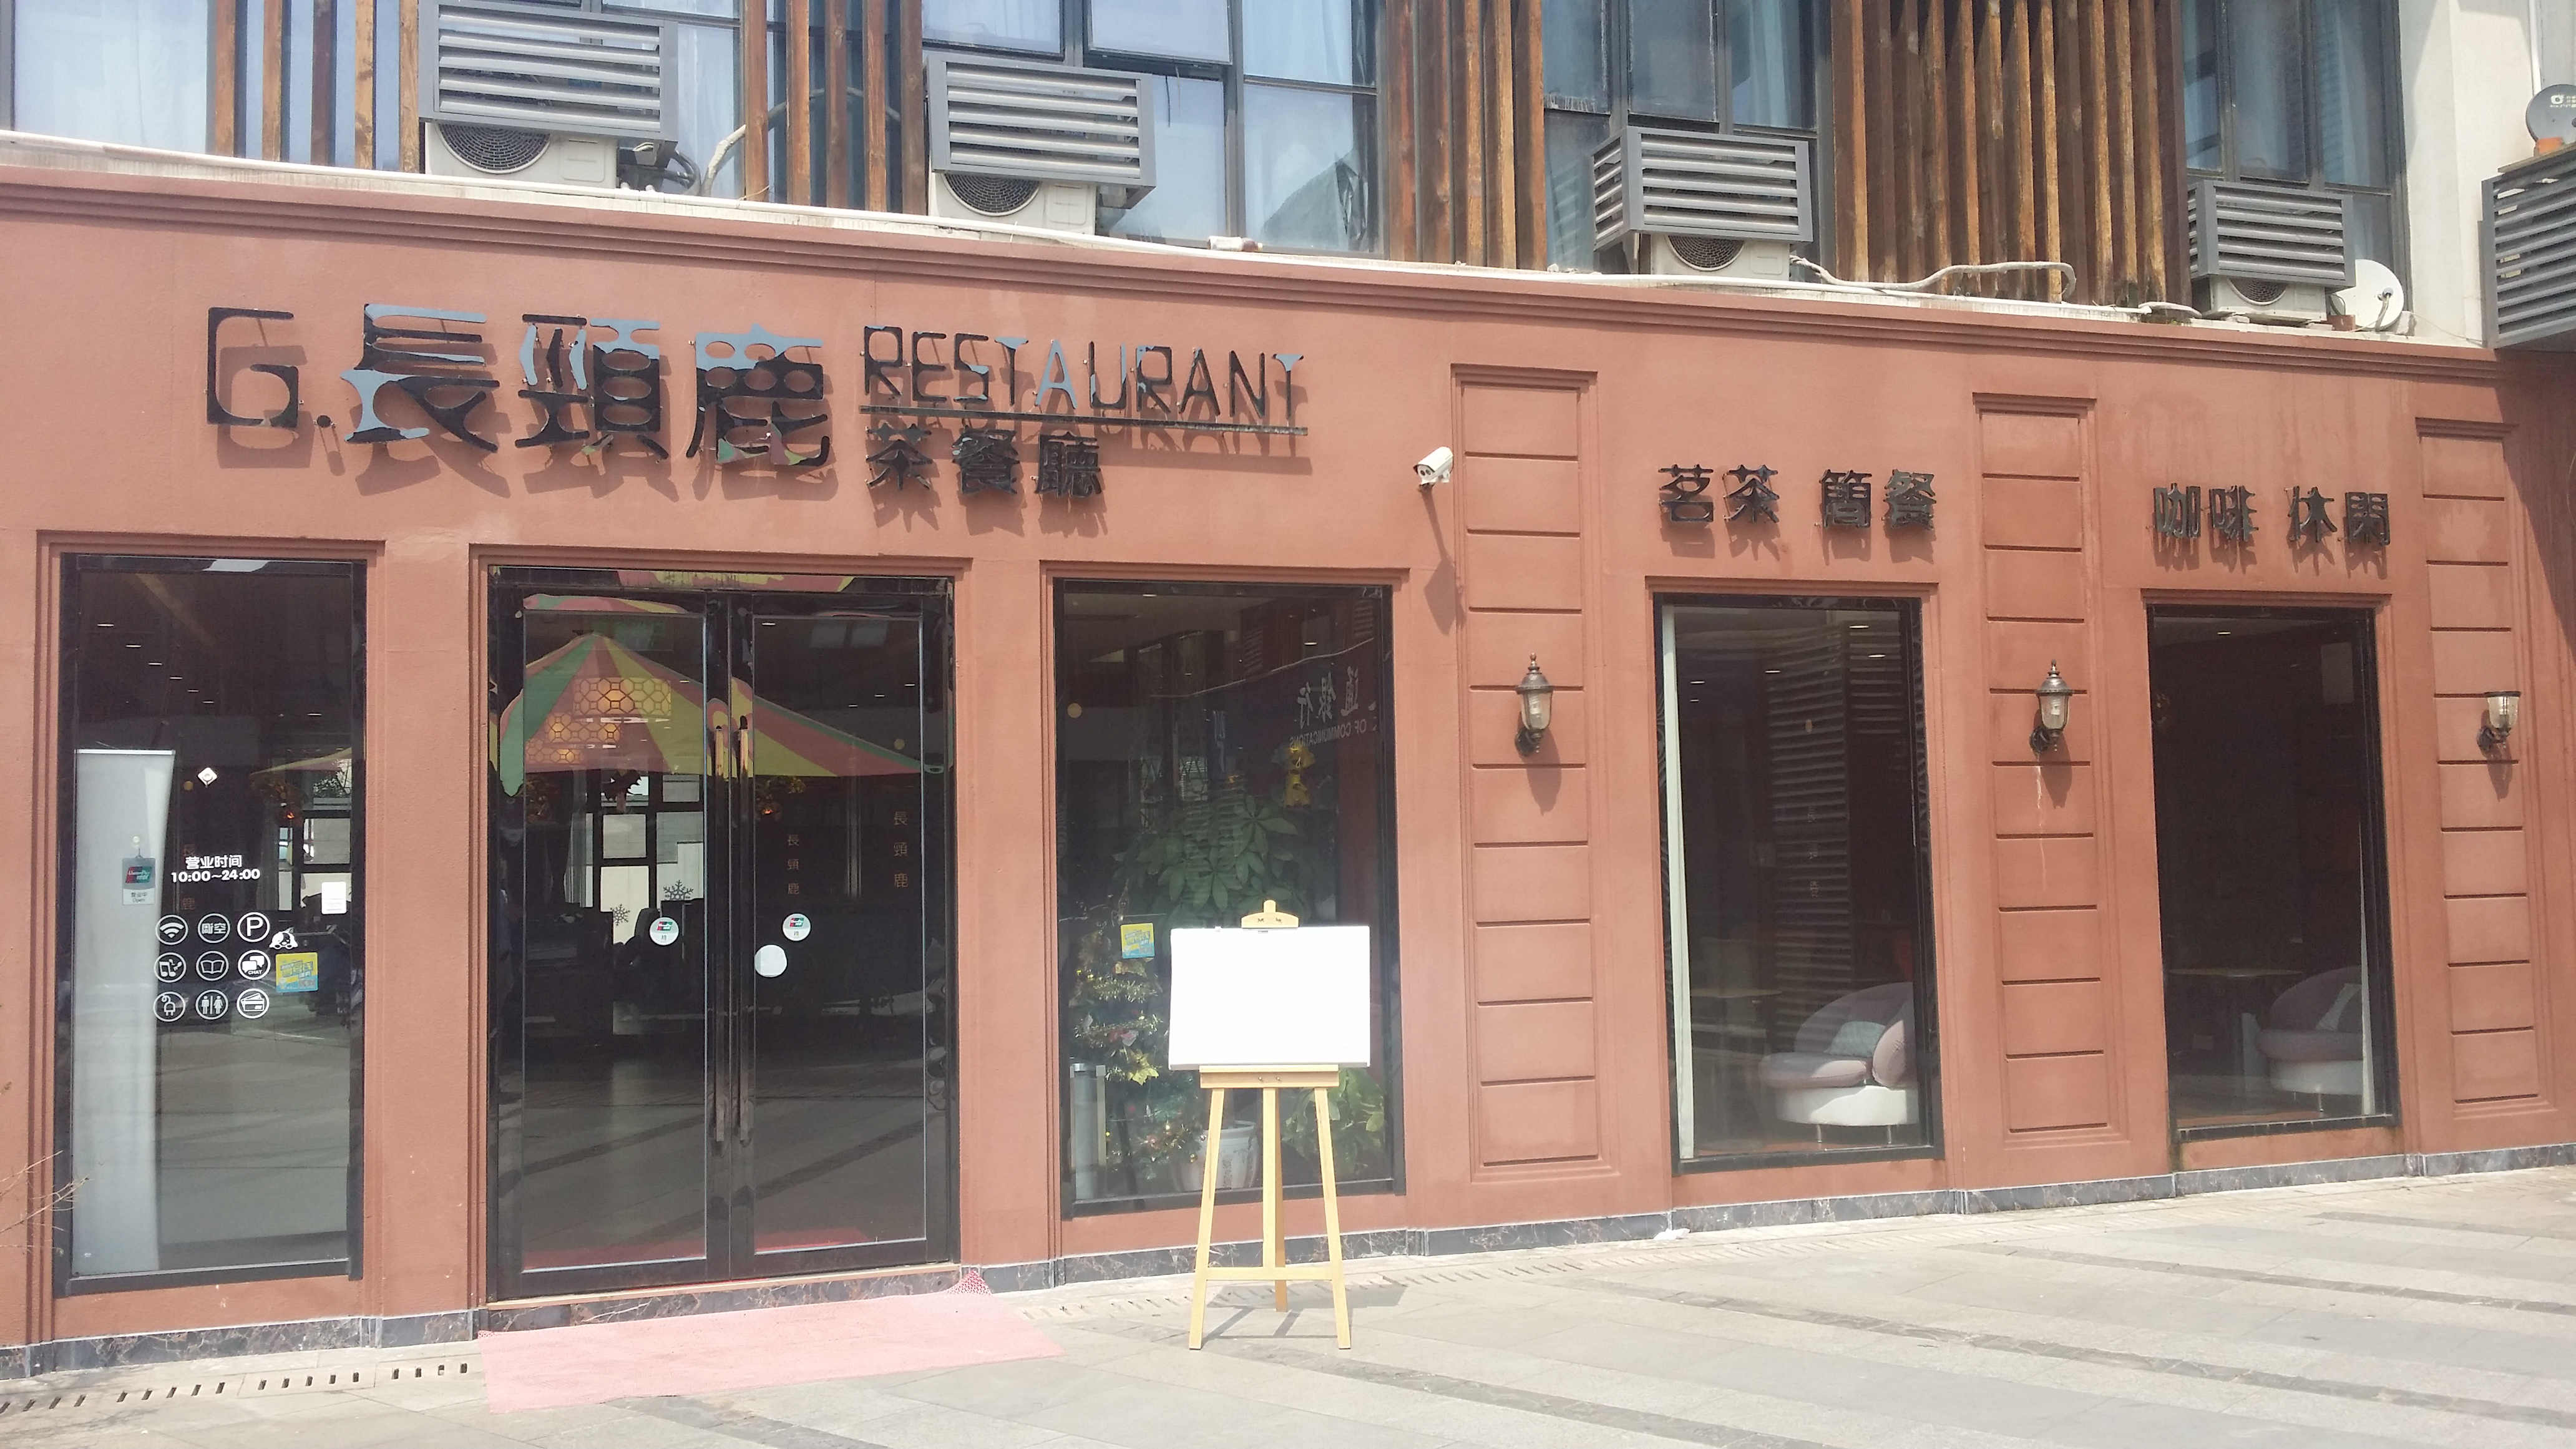
\includegraphics[scale=0.045]{travel_guide/rest.jpg}
\end{center}

\noindent This area also contains a ``Mickey Mouse bakery'',
which stocks pastries similar to the ones you might find in a 
Western bakery (just in case you get bored of the baozi
at breakfast in the hotel). There is also a pizza place in 
case you must eat something different than Chinese. 

There is also a smaller shopping area in the ``middle'' of
Tongwei road including some native restaurants. Some more
restaurants are on the opposite side of Houbiao\-ying Road. 

A smaller supermarket is at the end of Tongwei Road and a
bigger one, called Suguo Community Store, in the Xiamafang
area. For the latter, go down the steps in front of the KFC.
\end{itemize}

\section{Further Afield}

If you take the rather cheap and convenient metro, you are 
very quickly in the downtown area of Nanjing (see metro map in
Fig.~\ref{metronanjing} in the previous section). 

\begin{itemize}
\item\textbf{Shopping}\hspace{3mm}
The most serious shopping malls in Nanjing are in the area
around Xinjiekou and Daxinggong metro stations (on Line~2). Be
aware that especially in multi-brand shopping malls the
shopping goes like this: (1) You find something you like. (2)
You agree the prize with the shop-assistant. (3) You get a
piece of paper, which you need to take to a cashier nearby.
(4) You pay there, get another piece of paper, which you take
back to the shop-assistant, where you finally (5) receive your
goods. Another ``quirk'' of shopping in China is that when the
sale says ``80\% off'', for example, it is actually 20\% off,
meaning you pay only 80\% of the original price.

\item\textbf{Restaurants}\hspace{3mm}The most famous area
for restaurants in Nanjing is near the Confucius Temple, which
is near the Fuzimiao Metro Station on Line~3. There you
can find traditional-style houses and enjoy indigenous foods. 
There is also a myriad of restaurants in the Xinjiekou area. 

\item\textbf{Sight-Seeing}\hspace{3mm}Nanjing, being a former 
capital, possessed once one of the most impressive 
\textbf{\textit{city walls}}. 
Today you can see remainders at the North Gate near 
Zhonghuamen Metro Station on Line~1. From the station follow
the red line in the map below.

\begin{center}
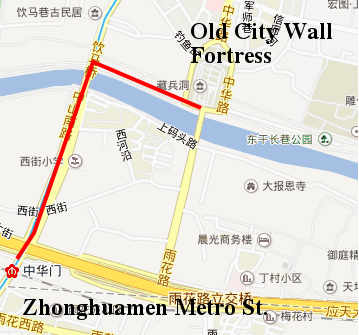
\includegraphics[scale=0.4]{travel_guide/map3.jpg}
\hspace{5mm}
\includegraphics[scale=0.3]{travel_guide/gate.jpg}
\end{center}


\noindent There is also another substantial section of the
remaining city wall visible in an area very close to the hotel
(you can see it from the hotel if you have a room sufficiently
high up): Walk the Houbiaoying Road towards the city centre;
once you traversed the river, bear right. You will see a tall
wall built of grey stones. At the beginning it is a restored
section, but further down the original wall starts (towards the
top-end in the map below).

\begin{center}
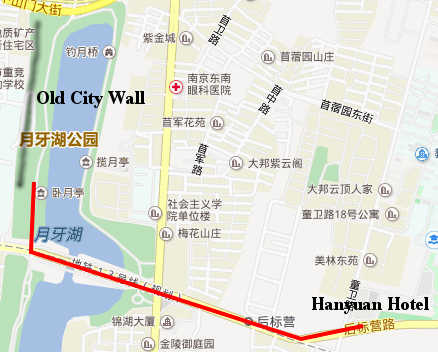
\includegraphics[scale=0.4]{travel_guide/map5.jpg}
\end{center}

Another scenic spot in Nanjing is the \textbf{\textit{Xuanwu
Lake}}, which is dotted with several beautiful small islands
and a good place to have a walk. You can reach the lake by
going to Xuanwumen Metro Station on Line~1. Xingyuan suggests
the walk indicated red below where you end up in from Jimingsi
Station on Line~3.


\begin{center}
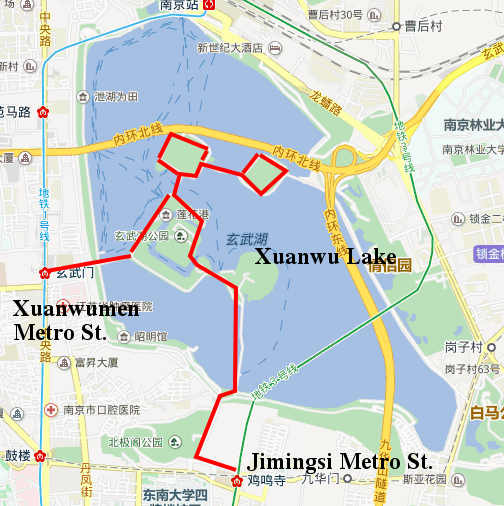
\includegraphics[scale=0.3]{travel_guide/map4.jpg}
\hspace{5mm}
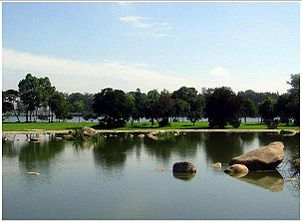
\includegraphics[scale=1.2]{travel_guide/xianwulake.jpg}
\end{center}

\noindent \textbf{\textit{Nanjing Museum}} is one of the
biggest museums in China and definitely worth a visit. For
this go to Minggugong Station on Line 2 (Minggugong is only 1
stop away from Muxuyuan; so you could also walk, if you are
very enthusiastic). Admission to the museum is from 9:00 untill 
16:00 and a visit is free. Some English information about 
current exhibitions is at \url{http://en.nanjingmuseum.com}. 
\medskip


\noindent The ultimate bird's-eye view of Nanjing you can have
from the \textbf{\textit{Zifeng Tower}}. For this you have to go to
Gulou Metro Station on Line~1. Zifeng Tower is just outside
the metro station. According to Wiki, Zifeng Tower is the
11th tallest building in the World (to compare, the Shard in
London is ranked 92nd and the Sears Tower in Chicago is 12th).
A ticket for the observation platform costs 66 RMB.
\end{itemize}

\section{Schedule of the Excursion\label{excursion}}

On Wednesday afternoon there will be the traditional
ITP-excursion, this time to a Chinese garden in Yangzhou and
to the Slender West Lake. You might like to note a few points:

\begin{itemize}
\item The conference session on Wednesday will end at 11:30,
      and you should finish lunch no later than 12:20 in order
      to get to the hotel lobby.
\item Boarding the shuttle bus is at 12:30 sharp!
\item The first leg of the bus journey takes roughly 1.5 hours
  to Ge Yuan Garden (meaning Bamboo Garden). This is a
  small garden in traditional Chinese style. We will be there
  for approximately 1h. You can find a short description at
  \url{https://en.wikipedia.org/wiki/Ge_Yuan_Garden}. 
  
\item After Ge Yuan, we are going to board the shuttle bus again 
  for the Slender West Lake. We are going to enter the Slender West 
  Lake area from its North Gate. The walking tour at Slender 
  West Lake will be lead by two guides speaking English.
  Wiki has some rudimentary information at
  \url{https://en.wikipedia.org/wiki/Slender_West_Lake}.
\item After the walk, we will board boats which will bring
  us to the South Gate of the lake.
\item The banquet restaurant (named Lion 
  Pavilion) is located on the campus 
  of Yangzhou University. It  will take us 5 minute walk 
    from the South Gate to get there.
\item We expect that the shuttle bus to brings us back starting 
  around 21:30 and we should be back in the hotel by 23:00.
\end{itemize}

\section{Restaurants}

China is of course famous for its food and restaurants. Below
we give an extremely selected list of a few restaurants, in
case you feel lost. One point to note, however, is that in
China meal times tend to happen earlier than elsewhere: for
example if you arrive at a restaurant at 13:00, you are
probably still fine for lunch, but arriving at 14:00 pushes
the envelop; similarly arriving for dinner at 20:00 at a
restaurant is fine, but 21:00 is too late. 

Surely you must have been to a Chinese restaurant in your home
town; but these restaurants have adapted a bit to Western
tastes. Therefore be aware of a few different customs: tip is
not expected. Also in many restaurants in China, you,
especially if you are in a large group, are expected to order
many small dishes, similar to how you would order Tapas, and
everybody in the group can then try all dishes. Similarly, the
idea of getting for every member of your group a separate bill
is \emph{not} supported by the Chinese way of eating out. If I
remember correctly, for tax-reasons restaurants have to pay
for every bill they hand out and thus under no circumstance
will they give several bills\ldots{}you have to come up with
your fellow dining-compadres with a way of how to split the
bill amongst yourselves. UPDATE: The rules about receipts have
changed in the past few months and restaurants actually can
give out more than one bill, as long as the amount on every
bill adds up to the whole amount. However, it is unclear
whether only ``upmarket'' restaurants are prepared to give out
several bills, or whether this is a universal possibility. So
far, we have only tried it in one instance. It is definitely
still an alien concept in China.

Many dishes in China are for carnivorous beings, but often
there are also completely vegetarian dishes---remember you
will normally be ordering many small dishes. Completely
vegetarian restaurants are rare in China.


\begin{itemize}
\item\textbf{Quanjude / Beijing Duck}\hspace{3mm}
Of course Beijing Roast Duck is not native to Nanjing, but it
is still very good: If you want to try it, you should
go to the Quanjude restaurant, which is very near the Xinjiekou Metro
Station (the entrance of the restaurant is shown on the right).

\begin{center}
\includegraphics[scale=0.16]{travel_guide/mapquanjude.jpg}
\hspace{5mm}
\includegraphics[scale=0.17]{travel_guide/quanjude.jpg}
\end{center}

\item\textbf{If you are lazy / exhausted, but still want to 
dine outside of the hotel}\dots{}%
If you feel like going to Hanyuan's own restaurant means you
have not been adventurous enough to see the ``outside'' world,
you can be a tad more adventurous by going to the 
DanFengYuLu (丹枫雨露)
restaurant. This restaurant is less than 5 minutes walk away 
on TongWei Road. It is a relative quiet restaurant
and has comfortable seats. The menu is in Chinese only, but it
contains lots of pictures. The restaurant is
located on the ``middle'' corner of TongWei Road (its entrance
is shown on the right). You have to go to the 2nd Floor.

\begin{center}
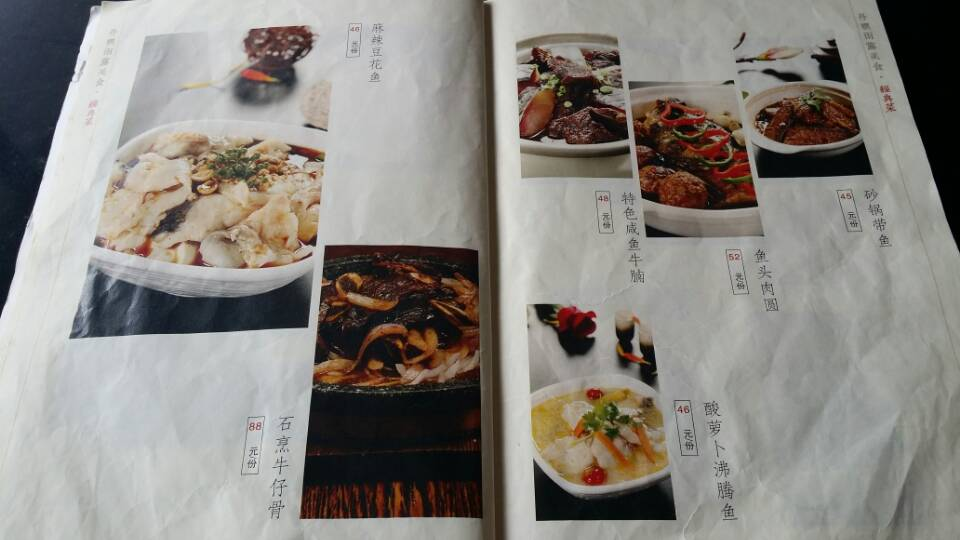
\includegraphics[scale=0.15]{travel_guide/menu.jpg}
\hspace{5mm}
\includegraphics[scale=0.11]{travel_guide/tonweirest.jpg}

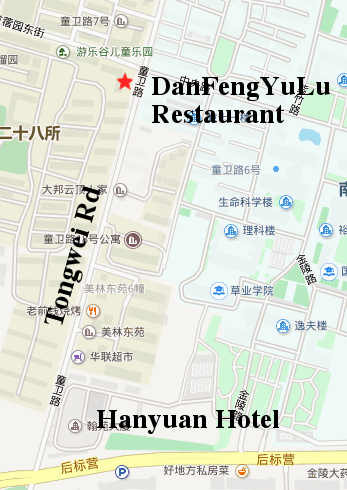
\includegraphics[scale=0.27]{travel_guide/map6.jpg}
\end{center}

In case you need it: this restaurant has a really free
wifi (no mobile needed)---wifi: dfyl128, password: 84865699.

\item\textbf{Two other restaurants near the hotel}\hspace{3mm}
On Houbiaoying Road (the ``big one'' in front of the hotel) 
are two restaurants next to each other---the entrances are


\begin{center}
\includegraphics[scale=0.04]{travel_guide/huobiaorest1.jpg}
\hspace{5mm}
\includegraphics[scale=0.04]{travel_guide/huobiaorest2.jpg}
\end{center}

The one on the right (JiangYanLou 江宴楼) is specialised in
fish/seafood dishes, while the other (YuPinZhouZhuang 御品周庄) is
more general fare.

\begin{center}
\includegraphics[scale=0.35]{travel_guide/map7.jpg}
\end{center}
\end{itemize}

\chapter{Return Home}

Every good time has to come to an end. We assume most people
have to leave via Nanjing Nan Train station (either to Nanjing
Lukou Airport or to Shanghai). If you have heavy luggage
the most sensible ways seems to take a taxi to Nanjing Nan, 
and then from there take the metro for example to Lukou 
Airport. Or go the whole way to the airport by taxi (remember to
make sure the taxi driver switches on the meter). Note that
the hotel usually does not call a taxi: you have to go to
the ``big road'' and hail one down yourself.\bigskip


\noindent
For Nanjing Nan show the taxi driver:
\begin{center}
\LARGE\addtolength{\fboxsep}{10mm}
\framebox{
\begin{tabular}{c}
司机师傅,请将我送到南京南火车站,谢谢。\medskip\\
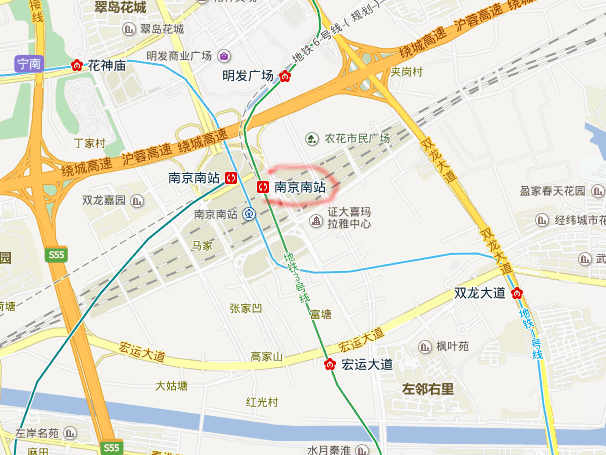
\includegraphics[scale=0.35]{travel_guide/nanjingnan.jpg}
\end{tabular}}
\end{center}

\subsection*{Train Tickets}

If you take the train to Shanghai, for example, especially 
if the train is on the weekend, it might be a good idea to
buy the ticket in advance. For this you have to go to the
train station and buy one at the ticket counter.


%For a bit of fun: the English description of some dishes 
%cannot be completely trusted:
%
%\begin{center}
%\includegraphics[scale=0.35]{travel_guide/fun.png}
%\end{center}

\newpage
\mbox{}\\[40mm]
\noindent The organising team wishes you a pleasant stay in 
Nanjing! If you need any help, please contact us.

\begin{center}
\begin{tabular}{ccc}
\includegraphics[scale=0.075]{pics/chunhan.jpg} &
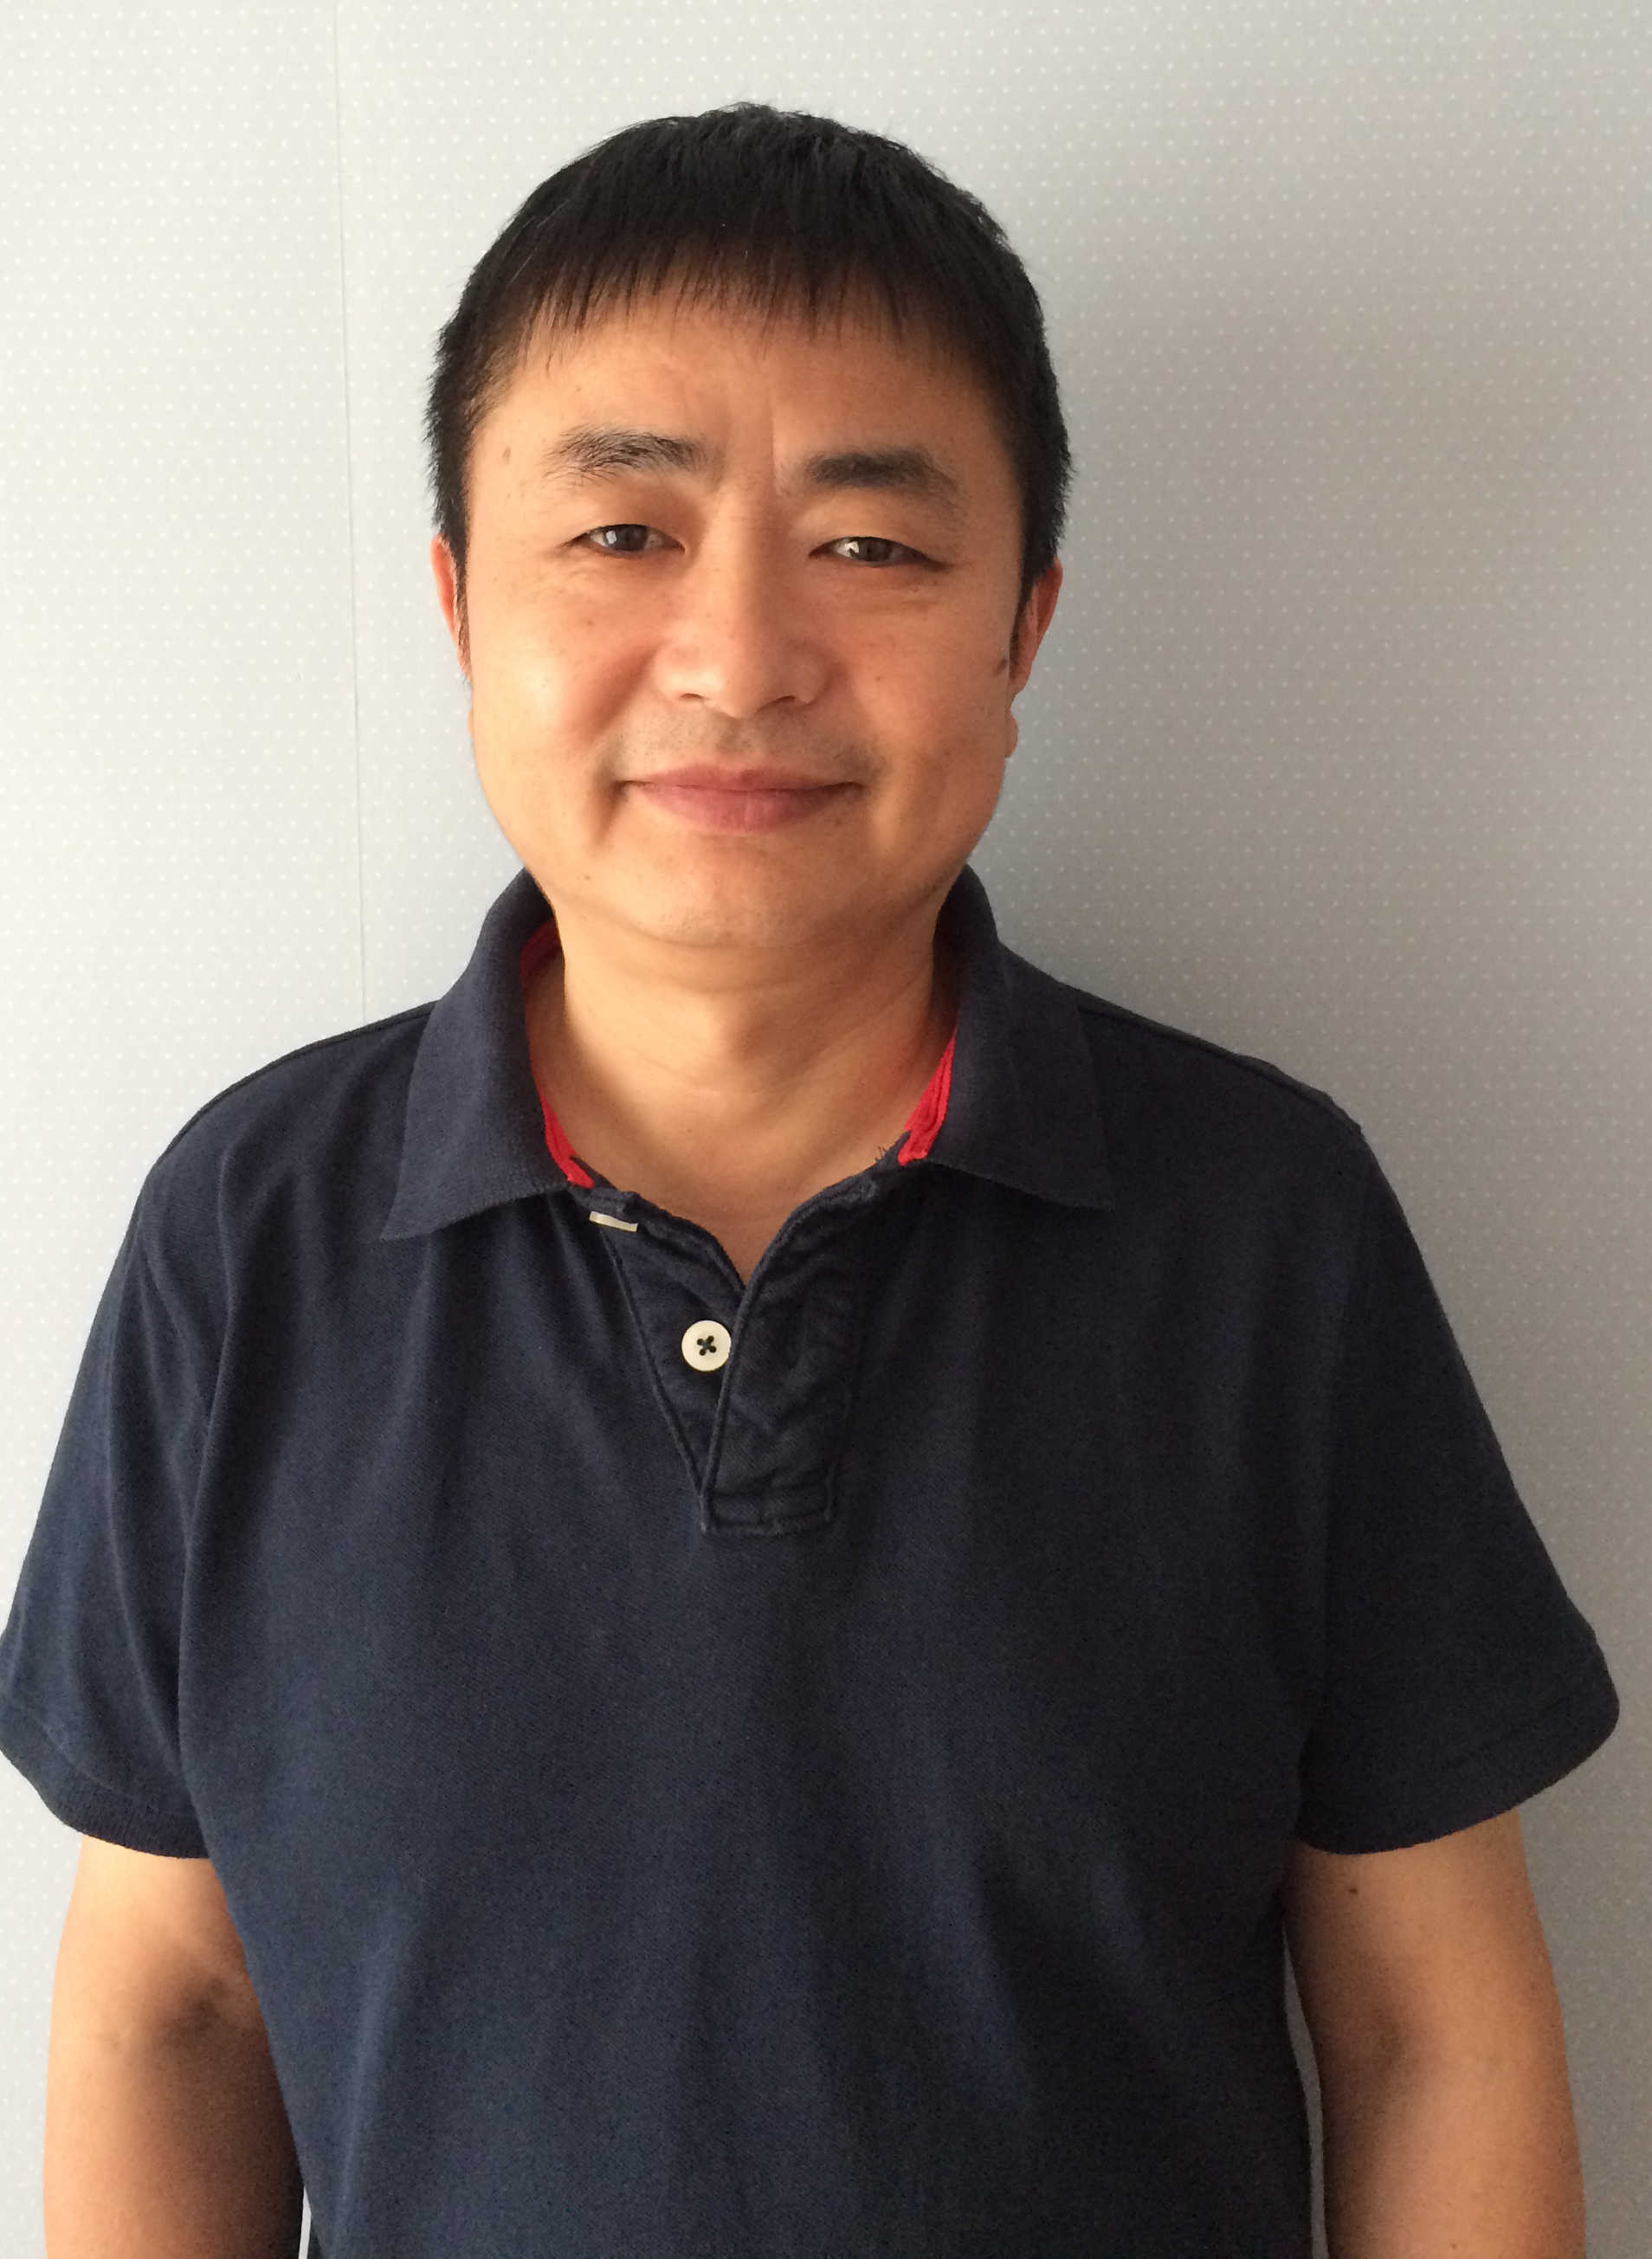
\includegraphics[scale=0.035]{pics/xingyuan.jpg} &
\includegraphics[scale=0.415]{pics/christian.jpg}\\
Chunhan Wu & Xingyuan Zhang & Christian Urban
\end{tabular}
\end{center}

\newlength{\cw}
\setlength{\cw}{100mm}
\newcolumntype{L}[1]{>{\raggedright\let\newline\\\arraybackslash\hspace{0pt}}m{#1}}

\begin{figure}[p]
\begin{center}
\rotatebox{90}{
\small
\begin{tabular}[t]{@{}*{2}{c @{\hspace{4mm}}} @{}}
 \mbox{}\\[-15mm]
 \begin{tabular}[t]{@{}|@{\hspace{0.5mm}}L{\cw}@{\hspace{0.5mm}}|}
  \multicolumn{1}{c}{\textbf{Monday (6th Floor)\smallskip}}\\
  \hline
  9:00 -- 10:00 (chairs: X.~Zhang, C.~Urban)\smallskip\\
  Short Intro Session\smallskip\\
  M.~Moscato, C.~Munoz, A.~Smith\\
  Affine Arithmetic and Applications to Real-Number Proving\\
  \hline
  \multicolumn{1}{@{}|l|@{}}{\hspace{-1mm}\cellcolor{blue!20}20 mins coffee break}\\
  \hline
  10:20 -- 11:10 (chair: T.~Nipkow)\smallskip\\
  J.~Hölzl, A.~Lochbihler, D.~Traytel\\ 
  A Formalized Hierarchy of Probabilistic System Types (Proof 
  Pearl)\smallskip\\
  F.~Immler\\ 
  A Verified Enclosure for the Lorenz Attractor (Rough 
  Diamond)\\
  \hline
  \multicolumn{1}{@{}|l|@{}}{\hspace{-1mm}\cellcolor{blue!20}20 mins coffee break}\\
  \hline
  11:30 -- 12:30 (chair: R.~Thiemann)\smallskip\\
  (moved to Thursday)\\ 
  \smallskip\\
  H.~Chan, M.~Norrish\\
  Mechanisation of AKS Algorithm: Part 1 – the Main Theorem\\
  \hline
  \multicolumn{1}{@{}|l|@{}}{\hspace{-1mm}\cellcolor{blue!20}2hs lunch break}\\
  \hline
  14:30 -- 15:30 (chair: R.~Kumar)\smallskip\\
  S.~Schneider, G.~Smolka, S.~Hack\\ 
  A First-Order Functional Intermediate Language for Verified 
  Compilers\smallskip\\
  A.~Fox\\ 
  Improved Tool Support for Machine-Code Decompilation in 
  HOL4\\
  \hline
  \multicolumn{1}{@{}|l|@{}}{\hspace{-1mm}\cellcolor{blue!20}30 mins coffee break}\\
  \hline
  16:00 -- 17:00 (chair:~H.~Herbelin)\smallskip\\
  F.~Besson, S.~Blazy, P.~Wilke\\ 
  A Concrete Memory Model for CompCert\smallskip\\
  T.~Tuerk, M.~Myreen, R.~Kumar\\
  Pattern Matches in HOL: A New Representation and Improved Code 
  Generation\\
  \hline
  \end{tabular} 
& \begin{tabular}[t]{|@{\hspace{0.5mm}}p{\cw}@{\hspace{0.5mm}}|}
  \multicolumn{1}{c}{\textbf{Tuesday (6th Floor)\smallskip}}\\
  \hline
  9:00 -- 10:00 (chair: M.~Norrish)\smallskip\\
  A.~Charguéraud, F.~Pottier\\
  Machine-Checked Verification of the Correctness and Amortized Complexity of an Efficient Union-Find 
  Implementation\smallskip\\
  T.~Nipkow\\ 
  Amortized Complexity Verified\\
  \hline
  \multicolumn{1}{@{}|l|@{}}{\hspace{-1mm}\cellcolor{blue!20}20 mins coffee break}\\
  \hline
  10:20 -- 11:10 (chair: J.~Urban)\smallskip\\
  S.~Blazy, D.~Demange, D.~Pichardie\\
  Validating Dominator Trees for a Fast, Verified Dominance 
  Test\smallskip\\
  A.~Lochbihler, A.~Maximova\\
  Stream Fusion for Isabelle'{}s Code Generator (Rough 
  Diamond)\\
  \hline
  \multicolumn{1}{@{}|l|@{}}{\hspace{-1mm}\cellcolor{blue!20}20 mins coffee break}\\
  \hline
  11:30 -- 12:30 (chair: X.~Zhang)\smallskip\\
  L.~Birkedal\\
  \textbf{Invited Talk}\\
  \hline
  \multicolumn{1}{@{}|l|@{}}{\hspace{-1mm}\cellcolor{blue!20}2hs lunch break}\\
  \hline
  14:30 -- 15:30 (chair: A.~Fox)\smallskip\\
  M.~Abdulaziz, M.~Norrish, C.~Gretton\\
  Verified Over-Approximation of the Diameters of Propositionally Factored Transition 
  Systems\smallskip\\
  T.~Prathamesh\\
  Formalizing Knot Theory in Isabelle/HOL\\
  \hline
  \multicolumn{1}{@{}|l|@{}}{\hspace{-1mm}\cellcolor{blue!20}30 mins coffee break}\\
  \hline
  16:00 -- 17:00 (chair: S.~Blazy)\smallskip\\
  S.~Schäfer, T.~Tebbi, G.~Smolka\\ 
  Autosubst: Reasoning with de Bruijn Terms and Parallel 
  Substitutions\smallskip\\
  P.~Maksimovic, A.~Schmitt\\
  HOCore in Coq\\
  \hline
  \multicolumn{1}{@{}|l|@{}}{\hspace{-1mm}\cellcolor{blue!20}short coffee break}\\
  \hline
  17:15 -- 18:00\smallskip\\
  \textbf{ITP Business Meeting}\\
  \hline
  \end{tabular}
\end{tabular}}
\end{center}
\end{figure}

\begin{figure}[p]
\begin{center}
\rotatebox{90}{
\small
\begin{tabular}[t]{@{} *{2}{c @{\hspace{4mm}}} @{}}
   \mbox{}\\[-20mm]
   \begin{tabular}[t]{|@{\hspace{0.5mm}}L{90mm}@{\hspace{0.5mm}}|}
   \multicolumn{1}{c}{\textbf{Wednesday (6th Floor)\smallskip}}\\
   \hline
   9:00 -- 10:00 (chair: A.~Charguéraud)\smallskip\\
   R.~Spadotti\\
   A Mechanized Theory of Regular Trees in Dependent Type 
   Theory\smallskip\\
   G.~Smolka, S.~Schäfer, C.~Doczkal\\
   Transfinite Constructions in Classical Type Theory\\
   \hline
   \multicolumn{1}{@{}|l|@{}}{\hspace{-1mm}\cellcolor{blue!20}30 mins coffee break}\\
   \hline
   10:30 -- 11:30 (chair: C.~Urban)\\
   M.~Norrish\\
   \textbf{Invited Talk}\\
   \hline
   \multicolumn{1}{@{}|l|@{}}{\hspace{-1mm}\cellcolor{blue!20}1h lunch break}\\
   \hline
   12:30 -- 22:30\smallskip\\
   Excursion to Ge Yuan Garden and Slender West Lake\smallskip\\
   The bus departs at 12:30 sharp from the hotel.\smallskip\\
   Dinner will be at the Lion Pavilion restaurant which is close
   to the Slender West Lake.\smallskip\\
   We expect to be back at the hotel around 22:30.\\
   \hline
   \end{tabular}
 & \begin{tabular}[t]{|@{\hspace{0.5mm}}L{130mm}@{\hspace{0.5mm}}|@{}}
   \multicolumn{1}{c}{\textbf{Thursday (6th Floor)\smallskip}}\\
   \hline
   9:00 -- 10:00 (chair: G.~Smolka)\smallskip\\
   B.~Fallenstein, R.~Kumar\\ 
   Proof-Producing Reflection for HOL, with an Application 
   to Model Polymorphism\smallskip\\ 
   O.~Kunčar, A.~Popescu\\ 
   A Consistent Foundation for Isabelle/HOL\\
   \hline
   \multicolumn{1}{@{}|l|@{}}{\hspace{-1mm}\cellcolor{blue!20}20 mins coffee break}\\
   \hline
   10:20 -- 11:10 (chair: S.~Boulm\'e)\smallskip\\
   Z.~Paraskevopoulou \textit{et al}\\ 
   Foundational Property-Based Testing\smallskip\\
   C.~Kaliszyk, J.~Urban, J.~Vyskocil\\ 
   Learning To Parse on Aligned Corpora (Rough Diamond)\\
   \hline
   \multicolumn{1}{@{}|l|@{}}{\hspace{-1mm}\cellcolor{blue!20}20 mins coffee break}\\
   \hline
   11:30 -- 12:30 (chair: D.~Pichardie)\smallskip\\
   F.~Sieczkowski, A.~Bizjak, L.~Birkedal\\ 
   ModuRes: A Coq Library for Modular Reasoning about Concurrent Higher-Order Imperative Programming 
   Languages\smallskip\\
   S.~Boulmé, A.~Maréchal\\
   Refinement to Certify Abstract Interpretations, Illustrated 
   on Linearization for Polyhedra\\
   \hline
   \multicolumn{1}{@{}|l|@{}}{\hspace{-1mm}\cellcolor{blue!20}2hs lunch break}\\
   \hline
   14:30 -- 15:30 (chair: C.~Wu)\smallskip\\
   C.~Sternagel, R.~Thiemann\\
   Deriving Comparators and Show-Functions in Isabelle/HOL\smallskip\\
   R.~Affeldt, J.~Garrigue\\
   Formalization of Error-Correcting Codes: from Hamming to Modern Coding 
   Theory\\
   \hline
   \multicolumn{1}{@{}|l|@{}}{\hspace{-1mm}\cellcolor{blue!20}30 mins coffee break}\\
   \hline
   16:00 -- 17:00 (chair: G.~Malecha)\smallskip\\
   P.~Lammich\\
   Refinement to Imperative/HOL\smallskip\\
   B.~Barras, C.~Tankink, E.~Tassi\\ 
   Asynchronous Processing of Coq Documents: 
   from the Kernel up to the User Interface\\
   \hline
   \multicolumn{1}{@{}|l|@{}}{\hspace{-1mm}\cellcolor{blue!20}short coffee break}\\
   \hline
   17:15 -- 18:15 (chair: M.~Moscato)\smallskip\\
   L.~Cruz-Filipe, P.~Schneider-Kamp\\
   Formalizing Size-Optimal Sorting Networks: Extracting a 
   Certified Proof Checker\smallskip\\
   A.~Anand, R.~Knepper\\ 
   ROSCoq: Robots Powered by Constructive Reals\\
   \hline
   \end{tabular} 
\end{tabular}}
\end{center}
\end{figure}

\end{document}  
